\section{Communication Hub}
The ESP32-S3-DevKitC-1 board, shown in Fig.~\ref{fig:ESP32-Photo}, was used as the central communication and control hub, enabling efficient data exchange between the two-wheeled mobile base, the ToF sensor array, and external systems such as computers, microcontrollers, mobile devices, or cloud services, as illustrated in Fig.~\ref{fig:system_flow_diagram}.

\subsection{Communication with the Mobile Base}
A custom communication protocol was developed to manage the exchange of control commands and telemetry data, which is structured around well-defined command and telemetry packets, implemented in \texttt{comm.hpp}. These packets support multiple data formats, ensuring compatibility with various communication protocols. Users can send commands to the mobile base and receive real-time telemetry feedback from the mobile base by using the provided member functions \texttt{comm.hpp} using communication protocols such as Inter-Integrated Circuit (I2C) and Universal Asynchronous Receiver-Transmitter (UART).

Inter-Integrated Circuit (I2C) communication is used for short-range, two-wire serial communication. The robot operates as an I2C slave with a predefined address (SLAVE\_ADDR = 8), allowing it to receive commands and transmit telemetry data over the I2C bus from the I2C master. The functions responsible for sending and receiving telemetry data are listed in Table~\ref{tab:i2c_methods}.

\begin{table}[h]
	\centering
	\caption{I2C Communication Methods}
	\begin{tabular}{|l|l|l|}
		\hline
		\textbf{Packet Type} & \textbf{Function} & \textbf{Description} \\ \hline
		\multirow{4}{*}{Command Packets} & \texttt{sendI2CBytes(addr)} & Sends command data as raw bytes to the address. \\ \cline{2-3}
		& \texttt{sendI2CASCII(addr)} & Sends command data as ASCII to the address. \\ \cline{2-3}
		& \texttt{readI2CBytes(addr)} & Reads command data as raw bytes from the address. \\ \cline{2-3}
		& \texttt{readI2CASCII(addr)} & Reads command data as ASCII from the address. \\ \hline
		\multirow{4}{*}{Telemetry Packets} & \texttt{sendI2CBytes()} & Sends telemetry data as raw bytes. \\ \cline{2-3}
		& \texttt{sendI2CASCII()} & Sends telemetry data as ASCII. \\ \cline{2-3}
		& \texttt{readI2CBytes(addr)} & Reads telemetry data as raw bytes from the address. \\ \cline{2-3}
		& \texttt{readI2CASCII(addr)} & Reads telemetry data as ASCII from the address. \\ \hline
	\end{tabular}
	\label{tab:i2c_methods}
\end{table}


The Universal Asynchronous Receiver-Transmitter (UART) protocol is used for serial communication. The UART communication is initialized at a baud rate of \texttt{9600}, which is used for the Bluetooth module used in this project~\cite{bluetooth_module}. The functions responsible for sending and receiving telemetry data are listed in Table~\ref{tab:uart_methods}. For this project, UART communication was used as it was found to be more reliable.
\begin{table}[h]
	\centering
	\caption{UART Communication Methods}
	\begin{tabular}{|l|l|l|}
		\hline
		\textbf{Packet Type} & \textbf{Function} & \textbf{Description} \\ \hline
		\multirow{4}{*}{Command Packets} & \texttt{readUartBytes()} & Reads command data as raw bytes. \\ \cline{2-3}
		& \texttt{readUartASCII()} & Reads command data as an ASCII string. \\ \cline{2-3}
		& \texttt{sendUartBytes()} & Sends command data as raw bytes. \\ \cline{2-3}
		& \texttt{sendUartASCII()} & Sends command data as an ASCII string. \\ \hline
		\multirow{4}{*}{Telemetry Packets} & \texttt{sendUartBytes()} & Sends telemetry data as raw bytes. \\ \cline{2-3}
		& \texttt{sendUartASCII()} & Sends telemetry data as an ASCII string. \\ \cline{2-3}
		& \texttt{readUartBytes()} & Reads telemetry data as raw bytes. \\ \cline{2-3}
		& \texttt{readUartASCII()} & Reads telemetry data as an ASCII string. \\ \hline
	\end{tabular}
	\label{tab:uart_methods}
\end{table}




\subsubsection{Sending Commands}
Users can send commands to control the robot’s movement, rotation, or stop function. Commands follow a predefined structured format and can be transmitted via either I2C or UART. The available commands are listed in Table~\ref{tab:commands}.

\textbf{ASCII Format}:
The commands sent in ASCII is formatted as a comma-separated string:
\begin{lstlisting}
	<command>,<command_value>,<command_speed>
\end{lstlisting}

\begin{table}[H]
	\centering
	\caption{List of Commands and Corresponding Values}
	\label{tab:commands}
	\begin{tabular}{|c|c|l|}
		\hline
		\textbf{Command} & \textbf{Value} & \textbf{Description} \\ \hline
		\texttt{Stop}     & 0              & Stops the robot's movement. \\
		& & \textit{Range: -32,768 to 32,767} \\ \hline
		\texttt{Move}     & 1              & Moves forward or backward (in cm) at a given speed. \\
		& & \textit{Range: -32,768 to 32,767} \\ \hline
		\texttt{Rotate}   & 2              & Rotates the robot by an angle (in degrees) at a given speed. \\
		& & \textit{Range: 0 to 359} \\ \hline
		\texttt{INVALID}  & 3              & Represents an invalid or unrecognized command. \\
		& & \textit{Range: -32,768 to 32,767} \\ \hline
	\end{tabular}
\end{table}

\textbf{Example Command:}
\begin{itemize}
	\item Stop the robot: \texttt{0,0,0}
	\item Move forward 100 cm at 50\% speed:  \texttt{1,100,50}
	\item Rotate 90° at 30 speed\%: \texttt{2,90,30}
\end{itemize}

\subsubsection{Receiving Telemetry Data}
The robot continuously monitors its state and environment using onboard sensors. This data is packaged into a structured format and transmitted back to the user for real-time monitoring and feedback. Telemetry data includes:
\begin{itemize}
	\item \textbf{Yaw Angle}: The robot's current orientation around the $y$-axis shown in Fig.~\ref{fig:pendulum_free_body_diagram} in degrees.
	\item \textbf{Distance Travelled}: The total distance travelled by the robot in centimetres.
	\item \textbf{Ultrasonic Distance}: The distance to the nearest obstacle, as measured by the ultrasonic sensor in centimetres.
	\item \textbf{Left IR Sensor}: Digital signal indicating detection of a persistent obstacle by the left sensor.
	\item \textbf{Right IR Sensor}: Digital signal indicating detection of a persistent obstacle by the right sensor.
	\item \textbf{Left Motor Encoder Pulses}: Total number of pulses recorded by the left wheel's encoder.
	\item \textbf{Right Motor Encoder Pulses}: Total number of pulses recorded by the right wheel's encoder.
\end{itemize}

\textbf{ASCII Format}:
The telemetry data received in ASCII is formatted as a comma-separated string:
\begin{lstlisting}[]
	<yaw_angle>,<distance_traveled>,<ultrasonic_distance>,
	<left_IR>,<right_IR>,<left_encoder>,<right_encoder>
\end{lstlisting}

\textbf{Example Output}:
\begin{lstlisting}[]
	45,200,30,1,0,1540,1572
\end{lstlisting}

This indicates:
\begin{itemize}
	\item A yaw angle of 45 degrees
	\item A total distance travelled of 200 cm
	\item An ultrasonic measures an obstacle at a distance of 30 cm ahead
	\item The left IR sensor detects an obstacle (1)
	\item The right IR sensor does not detect an obstacle (0)
	\item 1540 total encoder pulses on the left motor
	\item 1572 total encoder pulses on the right motor
\end{itemize}

\subsection{Communication with TerraRanger Multiflex}
The TerraRanger Multiflex communicates via UART, transmitting raw data for all eight sensors in ASCII format. The data string begins with the prefix 'MF' and is separated by tab characters, as shown below:

\begin{lstlisting}[]
	MF\t<Sensor 1>\t<Sensor 2>\t<Sensor 3>\t<Sensor 4>
	\t<Sensor 5>\t<Sensor 6>\t<Sensor 7>\t<Sensor 8>\r\n
\end{lstlisting}

In this format, each `<Sensor n>' represents the distance measured by the corresponding sensor in millimeters. The actual raw data received over UART from the TerraRanger Multiflex is illustrated in Fig.~\ref{fig:terra_received_data}.
\begin{figure}[H]
	\centering
	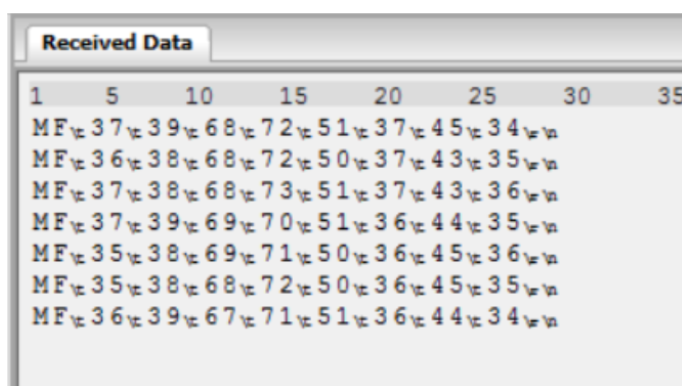
\includegraphics[height=6cm]{assets/terra_received_data.png}
	\caption{The received raw data from the TerraRanger Multiflex via UART.}
	\label{fig:terra_received_data}
\end{figure}

\subsection{Communication with External Systems}

The ESP32-S3 microcontroller is configured to operate in Soft Access Point (SoftAP) mode, enabling it to create a dedicated Wi-Fi network. This configuration allows external devices, such as a remote PC or handheld controller, to connect directly to the ESP32-S3 without requiring an intermediary router. Once connected, the ESP32-S3 facilitates two-way communication between the robot and the external system by transmitting telemetry data and receiving control commands, as illustrated in Fig.~\ref{fig:system_flow_diagram}.

\subsubsection{Telemetry Transmission}
To support real-time monitoring, the ESP32-S3 establishes a persistent TCP socket connection with a remote PC server. Sensor data—including measurements from the TerraRanger Multiflex (ToF sensors) and the mobile base—is read via UART interfaces. The received ASCII strings are then transmitted to the remote PC server. The system ensures low-latency updates and verifies the connection status before each transmission to maintain data integrity. Fig.~\ref{fig:live-data-streaming} illustrates the real-time visualization of the received telemetry in a polar plot.

\begin{figure}[H]
	\centering
	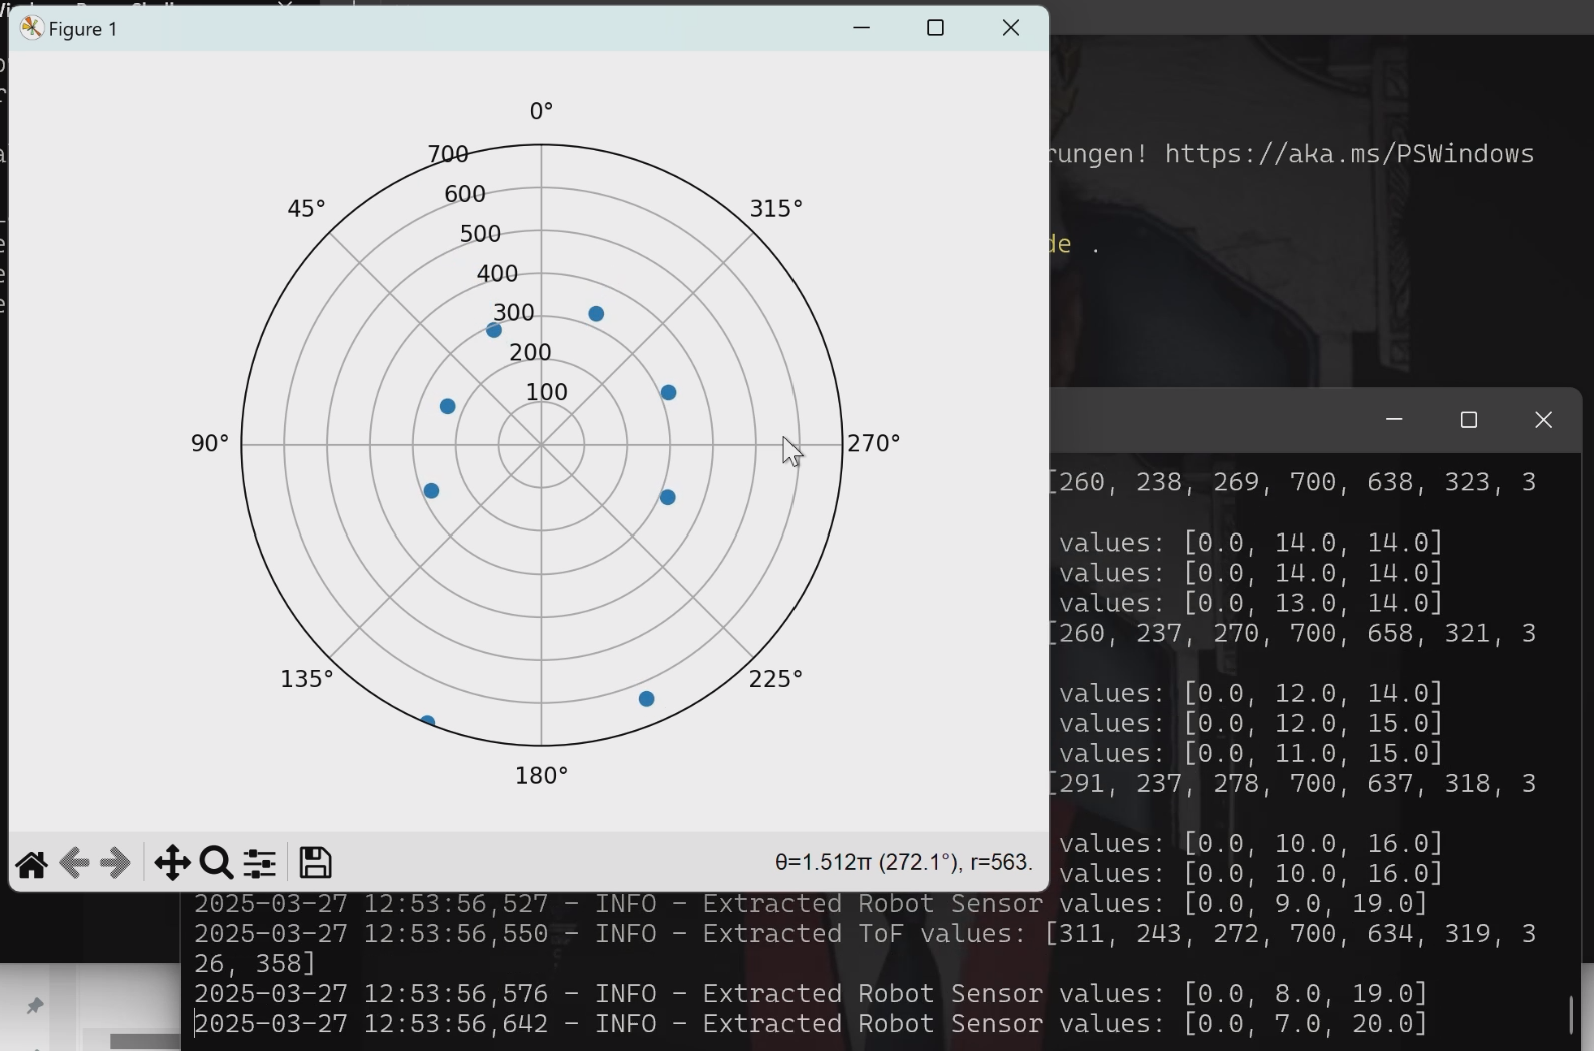
\includegraphics[height=9cm]{assets/LiveDataStreaming.png}
	\caption{Real-time sensor data visualization in a polar plot.}
	\label{fig:live-data-streaming}
\end{figure}

\subsubsection{Remote Command Reception and Execution}
The ESP32-S3 also supports command reception over TCP from a connected external device. This mechanism allows remote users to control the mobile robot in real time. The workflow for command handling is described below:

\begin{enumerate}
	\item \textbf{TCP Listening:} The ESP32-S3 continuously monitors its TCP server for incoming client connections.
	
	\item \textbf{Command Reception:} Once a client is connected, the ESP32-S3 reads the incoming ASCII-encoded command string. This string typically contains a command type (e.g., MOVE, ROTATE, STOP), a command value (e.g., angle or distance), and an associated speed parameter.
	
	\item \textbf{Parsing and Validation:} The received string is parsed to extract individual parameters. These parameters are then encapsulated into a structured data packet.
	
	\item \textbf{UART Transmission to Robot:} The formatted command packet is transmitted to the mobile base via UART.
	
	\item \textbf{Command Execution:} The ESP32-S3 supports the reception of remote control commands transmitted over a TCP socket in the form of structured ASCII strings. The available commands are listed in Table~\ref{tab:commands}. These commands are formatted as comma-separated values, representing the action to be performed, its magnitude, and the execution speed. A typical command string follows the pattern:
	\begin{center}
		\texttt{<COMMAND>,<VALUE>,<SPEED>}
	\end{center}
	
	\item \textbf{Client Disconnection:} After command execution, the ESP32-S3 acknowledges the command and closes the client connection.
\end{enumerate}

This bidirectional communication model enables seamless remote control and continuous monitoring, making it suitable for autonomous robotic applications and teleoperation scenarios.
